\scanpage{23}

\uline{Théorème 2} Soit $f:X\longrightarrow Y$ un
morphisme \deleted{\unsure{loc. de t.f.}} propre de
préschémas \inserted{\unsure{loc}} \unsure{noeths}, avec $Y$ intègre,
$y_0\in Y$, $y_1$ \deleted{\unsure{une générisation}}
\deleted{le \unsure{pt gén. de $Y$}}\inserted{le pt gén de $Y$}.
On suppose
\deleted{que l'on est dans le \unsure{cas des} \unsure{variétés}}
\deleted{\unsure{intég}}
\margin{\figure{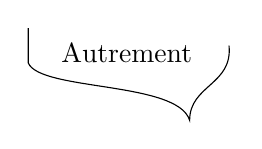
\begin{tikzpicture}[x=1cm,y=1cm]
\node at (0,0) {\deleted{\unsure{Autrement}}};
\draw (-1.25,.32) -- (-1.25,-.12) .. controls (-1.1,-.48) and (.65,-.35) .. (.8,-.85)
.. controls (.8,-.4) and (1.35,-.4) .. (1.3,.1);
\end{tikzpicture}}}

\margin{?}
\deleted{(a)} (a) $Y$ est [\unsure{géom.}$^{\unsure{t}}$] unibranche en $y_0$,
et les composantes irréductibles de
$X$ dominent $Y$.

\inserted{(b) les composantes irréductibles de}
\deleted{(b) $f$ est \unsure{universellement ouvert}.}
\deleted{\unsure{$f$}} \uline{$X_1$ sont} de dim $\geq h+1$, et $X_1$ est
connexe en dim $\geq h$.

Alors (les composantes irréductibles
de $X_0$ sont de dim $\geq h+1$) et
$X_0$ est \uline{connexe} en dim $\geq h$.

L'assertion \unsure{entre} parenthèses est
bien connue par le \unsure{théorème} des 2
dimensions, et n'utilise pas l'hypothèse
unibranche. Celle-ci sert uniquement
à appliquer le \uline{th. de \unsure{connexion|connexité}},
qui assure que $X_0$ est connexe.

\margin{22}
